\documentclass[twoside]{book}

% Packages required by doxygen
\usepackage{calc}
\usepackage{doxygen}
\usepackage{graphicx}
\usepackage[utf8]{inputenc}
\usepackage{makeidx}
\usepackage{multicol}
\usepackage{multirow}
\usepackage{textcomp}
\usepackage[table]{xcolor}

% Font selection
\usepackage[T1]{fontenc}
\usepackage{mathptmx}
\usepackage[scaled=.90]{helvet}
\usepackage{courier}
\usepackage{amssymb}
\usepackage{sectsty}
\renewcommand{\familydefault}{\sfdefault}
\allsectionsfont{%
  \fontseries{bc}\selectfont%
  \color{darkgray}%
}
\renewcommand{\DoxyLabelFont}{%
  \fontseries{bc}\selectfont%
  \color{darkgray}%
}

% Page & text layout
\usepackage{geometry}
\geometry{%
  a4paper,%
  top=2.5cm,%
  bottom=2.5cm,%
  left=2.5cm,%
  right=2.5cm%
}
\tolerance=750
\hfuzz=15pt
\hbadness=750
\setlength{\emergencystretch}{15pt}
\setlength{\parindent}{0cm}
\setlength{\parskip}{0.2cm}
\makeatletter
\renewcommand{\paragraph}{%
  \@startsection{paragraph}{4}{0ex}{-1.0ex}{1.0ex}{%
    \normalfont\normalsize\bfseries\SS@parafont%
  }%
}
\renewcommand{\subparagraph}{%
  \@startsection{subparagraph}{5}{0ex}{-1.0ex}{1.0ex}{%
    \normalfont\normalsize\bfseries\SS@subparafont%
  }%
}
\makeatother

% Headers & footers
\usepackage{fancyhdr}
\pagestyle{fancyplain}
\fancyhead[LE]{\fancyplain{}{\bfseries\thepage}}
\fancyhead[CE]{\fancyplain{}{}}
\fancyhead[RE]{\fancyplain{}{\bfseries\leftmark}}
\fancyhead[LO]{\fancyplain{}{\bfseries\rightmark}}
\fancyhead[CO]{\fancyplain{}{}}
\fancyhead[RO]{\fancyplain{}{\bfseries\thepage}}
\fancyfoot[LE]{\fancyplain{}{}}
\fancyfoot[CE]{\fancyplain{}{}}
\fancyfoot[RE]{\fancyplain{}{\bfseries\scriptsize Generated on Tue Jun 10 2014 10\-:02\-:03 for Checkers A\-I by Doxygen }}
\fancyfoot[LO]{\fancyplain{}{\bfseries\scriptsize Generated on Tue Jun 10 2014 10\-:02\-:03 for Checkers A\-I by Doxygen }}
\fancyfoot[CO]{\fancyplain{}{}}
\fancyfoot[RO]{\fancyplain{}{}}
\renewcommand{\footrulewidth}{0.4pt}
\renewcommand{\chaptermark}[1]{%
  \markboth{#1}{}%
}
\renewcommand{\sectionmark}[1]{%
  \markright{\thesection\ #1}%
}

% Indices & bibliography
\usepackage{natbib}
\usepackage[titles]{tocloft}
\setcounter{tocdepth}{3}
\setcounter{secnumdepth}{5}
\makeindex

% Hyperlinks (required, but should be loaded last)
\usepackage{ifpdf}
\ifpdf
  \usepackage[pdftex,pagebackref=true]{hyperref}
\else
  \usepackage[ps2pdf,pagebackref=true]{hyperref}
\fi
\hypersetup{%
  colorlinks=true,%
  linkcolor=blue,%
  citecolor=blue,%
  unicode%
}

% Custom commands
\newcommand{\clearemptydoublepage}{%
  \newpage{\pagestyle{empty}\cleardoublepage}%
}


%===== C O N T E N T S =====

\begin{document}

% Titlepage & ToC
\hypersetup{pageanchor=false}
\pagenumbering{roman}
\begin{titlepage}
\vspace*{7cm}
\begin{center}%
{\Large Checkers A\-I }\\
\vspace*{1cm}
{\large Generated by Doxygen 1.8.6}\\
\vspace*{0.5cm}
{\small Tue Jun 10 2014 10:02:03}\\
\end{center}
\end{titlepage}
\clearemptydoublepage
\tableofcontents
\clearemptydoublepage
\pagenumbering{arabic}
\hypersetup{pageanchor=true}

%--- Begin generated contents ---
\chapter{Alec Farfan}
\label{index}\hypertarget{index}{}Name\-: Alec Farfan \par
 Date\-: 06/03/14 \par
 Purpose\-: Project I\-I (Checkers A\-I) \par
 \par
 Checkers (also known as Draughts) is a two person strategy game where players compete against each other by moving along a diagonal axis, capturing each others pieces by jumping over them. The object of the game is to capture all the opponents game pieces or block them from being able to make any valid moves. The game is played on an 8 x 8 grid with alternating white and black squares across each row. The game checkers is what is called a solved game, which means that a particular game's outcome can be predicted from any position granted both players play with optimum strategy. Checkers A\-Is like Chinook can play better than the top ranked human players. 
\chapter{Hierarchical Index}
\section{Class Hierarchy}
This inheritance list is sorted roughly, but not completely, alphabetically\-:\begin{DoxyCompactList}
\item \contentsline{section}{Board}{\pageref{class_board}}{}
\begin{DoxyCompactList}
\item \contentsline{section}{State}{\pageref{class_state}}{}
\end{DoxyCompactList}
\item \contentsline{section}{Game\-Piece}{\pageref{class_game_piece}}{}
\begin{DoxyCompactList}
\item \contentsline{section}{King}{\pageref{class_king}}{}
\item \contentsline{section}{Reg\-Black}{\pageref{class_reg_black}}{}
\item \contentsline{section}{Reg\-White}{\pageref{class_reg_white}}{}
\end{DoxyCompactList}
\item \contentsline{section}{Game\-Tree}{\pageref{class_game_tree}}{}
\item \contentsline{section}{Queue$<$ T $>$}{\pageref{class_queue}}{}
\item \contentsline{section}{Queue$<$ std\-:\-:string $>$}{\pageref{class_queue}}{}
\item \contentsline{section}{Stack$<$ T $>$}{\pageref{class_stack}}{}
\end{DoxyCompactList}

\chapter{Class Index}
\section{Class List}
Here are the classes, structs, unions and interfaces with brief descriptions\-:\begin{DoxyCompactList}
\item\contentsline{section}{\hyperlink{class_board}{Board} }{\pageref{class_board}}{}
\item\contentsline{section}{\hyperlink{class_game_piece}{Game\-Piece} }{\pageref{class_game_piece}}{}
\item\contentsline{section}{\hyperlink{class_game_tree}{Game\-Tree} }{\pageref{class_game_tree}}{}
\item\contentsline{section}{\hyperlink{class_king}{King} }{\pageref{class_king}}{}
\item\contentsline{section}{\hyperlink{class_queue}{Queue$<$ T $>$} }{\pageref{class_queue}}{}
\item\contentsline{section}{\hyperlink{class_reg_black}{Reg\-Black} }{\pageref{class_reg_black}}{}
\item\contentsline{section}{\hyperlink{class_reg_white}{Reg\-White} }{\pageref{class_reg_white}}{}
\item\contentsline{section}{\hyperlink{class_stack}{Stack$<$ T $>$} }{\pageref{class_stack}}{}
\item\contentsline{section}{\hyperlink{class_state}{State} }{\pageref{class_state}}{}
\end{DoxyCompactList}

\chapter{Class Documentation}
\hypertarget{class_board}{\section{Board Class Reference}
\label{class_board}\index{Board@{Board}}
}


{\ttfamily \#include \char`\"{}Board.\-h\char`\"{}}

Inheritance diagram for Board\-:\begin{figure}[H]
\begin{center}
\leavevmode
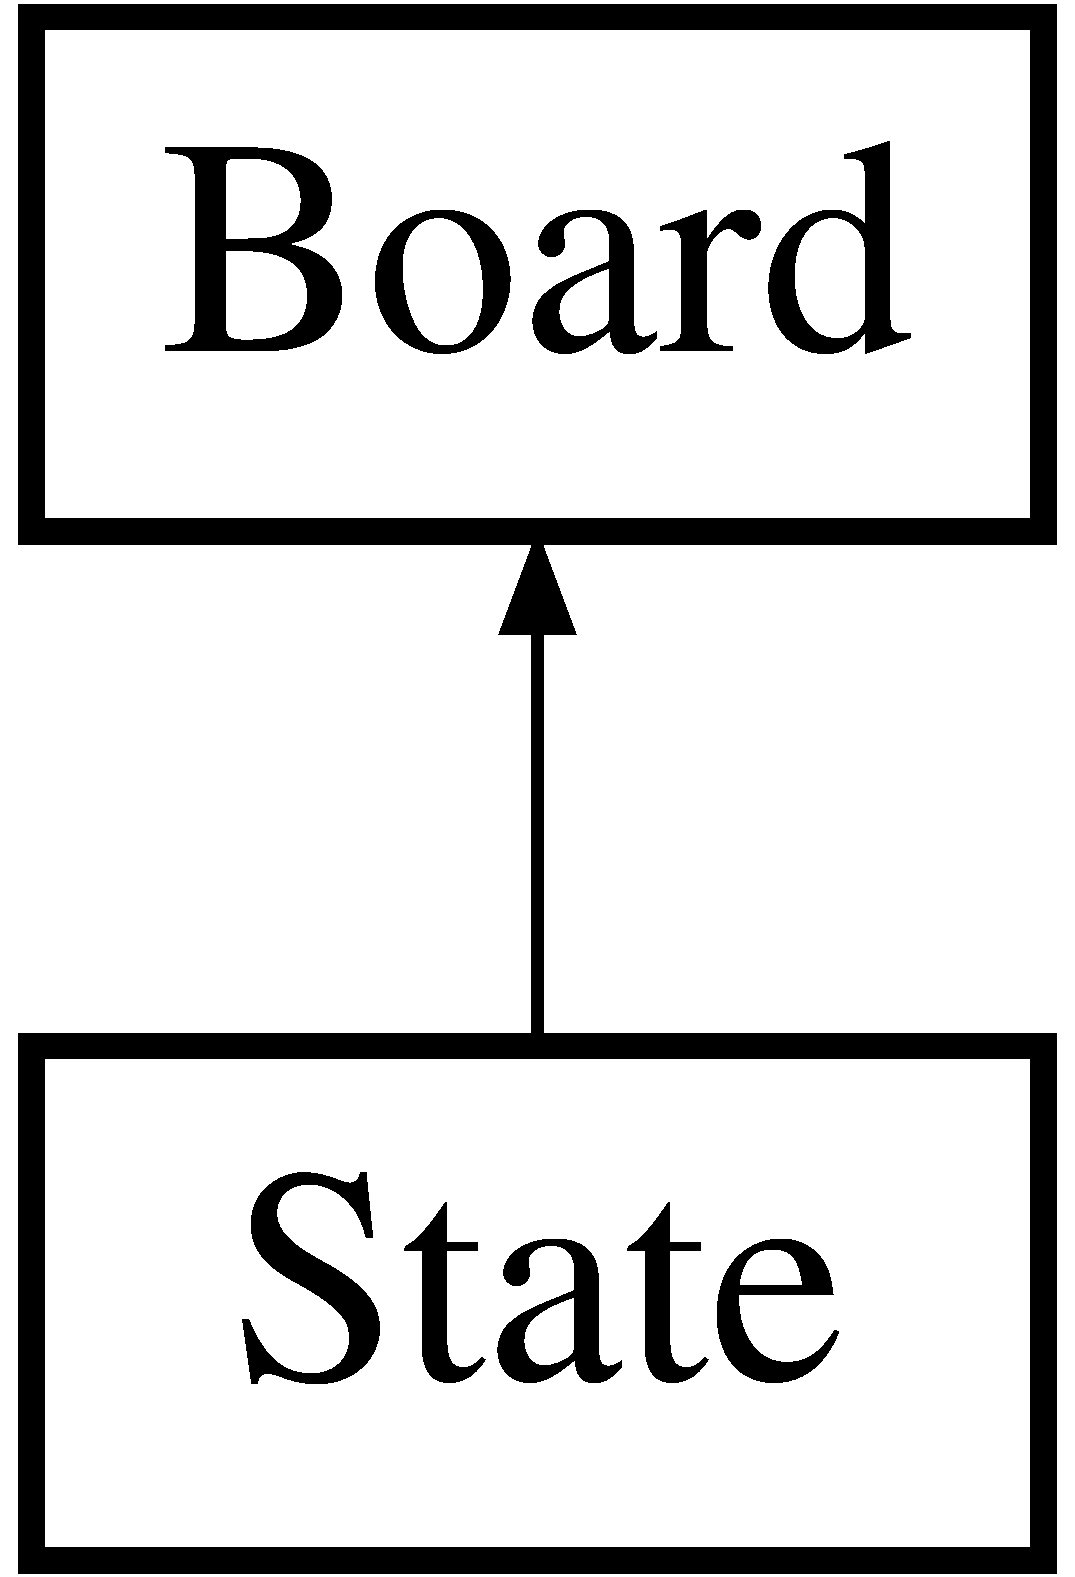
\includegraphics[height=2.000000cm]{class_board}
\end{center}
\end{figure}
\subsection*{Public Member Functions}
\begin{DoxyCompactItemize}
\item 
\hyperlink{class_board_a9ee491d4fea680cf69b033374a9fdfcb}{Board} ()
\item 
\hyperlink{class_board_ab7d6d506f23ebce7179e88ce9f15eb6c}{Board} (\hyperlink{class_board}{Board} \&)
\item 
void \hyperlink{class_board_a8b7e2a5722a7ec5527d853fb43494aa3}{display} (char, char, int, int)
\item 
int \hyperlink{class_board_a72a4e5c6530afafb6617e044f39ce7f2}{get\-Choice} (std\-::string, int)
\item 
bool \hyperlink{class_board_acaacbbbe559e3648019e1eddc7c94a1b}{remove} (\hyperlink{class_board}{Board} \&, char, int, int, int \&)
\item 
void \hyperlink{class_board_a94f4902b3feba31138f01f16dc1148c1}{chk\-Win} (bool \&, int, int)
\end{DoxyCompactItemize}
\subsection*{Static Public Member Functions}
\begin{DoxyCompactItemize}
\item 
static void \hyperlink{class_board_a6c43132a8b631bda53df49dce4ba93db}{swap} (char \&, char \&)
\end{DoxyCompactItemize}
\subsection*{Protected Attributes}
\begin{DoxyCompactItemize}
\item 
\hypertarget{class_board_ac3681603c987fc26f8c92f686f6771f3}{char {\bfseries square} \mbox{[}65\mbox{]}}\label{class_board_ac3681603c987fc26f8c92f686f6771f3}

\end{DoxyCompactItemize}
\subsection*{Friends}
\begin{DoxyCompactItemize}
\item 
\hypertarget{class_board_ab995b607204a3fc16276228c50c7784f}{class {\bfseries Game\-Piece}}\label{class_board_ab995b607204a3fc16276228c50c7784f}

\item 
\hypertarget{class_board_a0939d48ce34dc3c2c43e985becde0059}{class {\bfseries Reg\-White}}\label{class_board_a0939d48ce34dc3c2c43e985becde0059}

\item 
\hypertarget{class_board_a13f65c58c2d8e57345d4d58a043a27d0}{class {\bfseries Reg\-Black}}\label{class_board_a13f65c58c2d8e57345d4d58a043a27d0}

\item 
\hypertarget{class_board_aa6cf82643411ed9e0232886e11bd82f3}{class {\bfseries King}}\label{class_board_aa6cf82643411ed9e0232886e11bd82f3}

\end{DoxyCompactItemize}


\subsection{Detailed Description}
The \hyperlink{class_board}{Board} class represents the physical checkerboard that a game of checkers is usually played on. To mimic a checkerboard's black and white squares, plus + and minus -\/ characters are printed to the board. The classes representing black checkers, white checkers, and king checkers are friends with this class. The board is changed by these objects by the characters held within them, an object doesn't actually need to be placed on the board. The \hyperlink{class_board}{Board} class is responsible for all the tasks involving searching the board as well as making changes to it. 

\subsection{Constructor \& Destructor Documentation}
\hypertarget{class_board_a9ee491d4fea680cf69b033374a9fdfcb}{\index{Board@{Board}!Board@{Board}}
\index{Board@{Board}!Board@{Board}}
\subsubsection[{Board}]{\setlength{\rightskip}{0pt plus 5cm}Board\-::\-Board (
\begin{DoxyParamCaption}
{}
\end{DoxyParamCaption}
)}}\label{class_board_a9ee491d4fea680cf69b033374a9fdfcb}
This function is the constructor for the \hyperlink{class_board}{Board} class. Plus '+' and minus '-\/' signs are painted across the board in a checkerboard image with 'O' and ascii 149 representing the white and black checkers respectively.\hypertarget{class_board_ab7d6d506f23ebce7179e88ce9f15eb6c}{\index{Board@{Board}!Board@{Board}}
\index{Board@{Board}!Board@{Board}}
\subsubsection[{Board}]{\setlength{\rightskip}{0pt plus 5cm}Board\-::\-Board (
\begin{DoxyParamCaption}
\item[{{\bf Board} \&}]{obj}
\end{DoxyParamCaption}
)}}\label{class_board_ab7d6d506f23ebce7179e88ce9f15eb6c}
This function is a copy constructor for the \hyperlink{class_board}{Board} class. This function is mainly used to instantiate \hyperlink{class_state}{State} objects which are derived from this class.

\subsection{Member Function Documentation}
\hypertarget{class_board_a94f4902b3feba31138f01f16dc1148c1}{\index{Board@{Board}!chk\-Win@{chk\-Win}}
\index{chk\-Win@{chk\-Win}!Board@{Board}}
\subsubsection[{chk\-Win}]{\setlength{\rightskip}{0pt plus 5cm}void Board\-::chk\-Win (
\begin{DoxyParamCaption}
\item[{bool \&}]{win, }
\item[{int}]{p1, }
\item[{int}]{p2}
\end{DoxyParamCaption}
)}}\label{class_board_a94f4902b3feba31138f01f16dc1148c1}
This function checks to see if the game has been won by viewing the count of both of the players pieces. If the game is over the message stating who the winner is gets printed to the screen.\hypertarget{class_board_a8b7e2a5722a7ec5527d853fb43494aa3}{\index{Board@{Board}!display@{display}}
\index{display@{display}!Board@{Board}}
\subsubsection[{display}]{\setlength{\rightskip}{0pt plus 5cm}void Board\-::display (
\begin{DoxyParamCaption}
\item[{char}]{a, }
\item[{char}]{b, }
\item[{int}]{p1\-C, }
\item[{int}]{p2\-C}
\end{DoxyParamCaption}
)}}\label{class_board_a8b7e2a5722a7ec5527d853fb43494aa3}
Function displays a checkerboard made by piecing together strings and nesting an element of the array in each of the squares. Around the board a letter/number coordinate system is drawn to allow the users to point to a game square. To the right of the game board a scoreboard is printed showing current statuses of the game.\hypertarget{class_board_a72a4e5c6530afafb6617e044f39ce7f2}{\index{Board@{Board}!get\-Choice@{get\-Choice}}
\index{get\-Choice@{get\-Choice}!Board@{Board}}
\subsubsection[{get\-Choice}]{\setlength{\rightskip}{0pt plus 5cm}int Board\-::get\-Choice (
\begin{DoxyParamCaption}
\item[{std\-::string}]{, }
\item[{int}]{}
\end{DoxyParamCaption}
)}}\label{class_board_a72a4e5c6530afafb6617e044f39ce7f2}
This function reads in a letter/number coordinate choice from the user which is then copied into a character array to be manipulated and tested for validity. The type of validity this function is responsible for checking is in terms of data format ie. proper size, proper letter/number entry, ect. The val\-Choice and val\-Move functions are responsible for testing validity in terms of what is legal in the game of checkers.\hypertarget{class_board_acaacbbbe559e3648019e1eddc7c94a1b}{\index{Board@{Board}!remove@{remove}}
\index{remove@{remove}!Board@{Board}}
\subsubsection[{remove}]{\setlength{\rightskip}{0pt plus 5cm}bool Board\-::remove (
\begin{DoxyParamCaption}
\item[{{\bf Board} \&}]{game\-Board, }
\item[{char}]{b\-Piece, }
\item[{int}]{coord\-S, }
\item[{int}]{coord\-M, }
\item[{int \&}]{count}
\end{DoxyParamCaption}
)}}\label{class_board_acaacbbbe559e3648019e1eddc7c94a1b}
This function removes a game piece that has been jumped and captured. The array element holding the game piece that needs to be removed can be found by taking the average of the coordinate of the selected game piece and the coordinate of empty game square chosen to move the piece to.\hypertarget{class_board_a6c43132a8b631bda53df49dce4ba93db}{\index{Board@{Board}!swap@{swap}}
\index{swap@{swap}!Board@{Board}}
\subsubsection[{swap}]{\setlength{\rightskip}{0pt plus 5cm}void Board\-::swap (
\begin{DoxyParamCaption}
\item[{char \&}]{a, }
\item[{char \&}]{b}
\end{DoxyParamCaption}
)\hspace{0.3cm}{\ttfamily [static]}}}\label{class_board_a6c43132a8b631bda53df49dce4ba93db}
This function updates the display of the board by swapping the character representing a player's game piece which has been selected, with the character representing the empty game square that has been chosen to move the selected game piece to.

The documentation for this class was generated from the following files\-:\begin{DoxyCompactItemize}
\item 
C\-:/\-Users/\-Alec/\-Desktop/\-Project\-\_\-2/\-Checkers/Board.\-h\item 
C\-:/\-Users/\-Alec/\-Desktop/\-Project\-\_\-2/\-Checkers/Board.\-cpp\end{DoxyCompactItemize}

\hypertarget{class_game_piece}{\section{Game\-Piece Class Reference}
\label{class_game_piece}\index{Game\-Piece@{Game\-Piece}}
}


{\ttfamily \#include \char`\"{}Game\-Piece.\-h\char`\"{}}

Inheritance diagram for Game\-Piece\-:\begin{figure}[H]
\begin{center}
\leavevmode
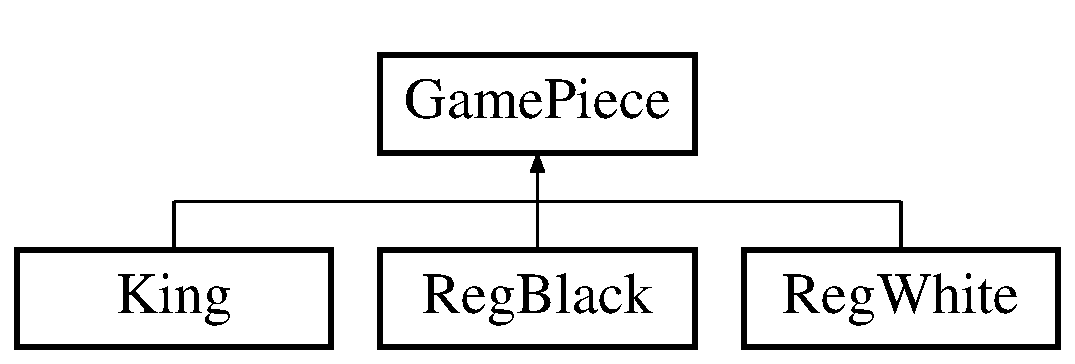
\includegraphics[height=2.000000cm]{class_game_piece}
\end{center}
\end{figure}
\subsection*{Public Member Functions}
\begin{DoxyCompactItemize}
\item 
\hypertarget{class_game_piece_a595e9a724c19032fddf1b7b09e3a2bf3}{virtual void {\bfseries val\-Pick} (string, \hyperlink{class_board}{Board} \&, char, char, char \&, int \&)=0}\label{class_game_piece_a595e9a724c19032fddf1b7b09e3a2bf3}

\item 
\hypertarget{class_game_piece_af13687186a04d74491d55b9b621b6160}{virtual bool {\bfseries chk\-Pick} (\hyperlink{class_board}{Board} \&, char, char, char \&, int)=0}\label{class_game_piece_af13687186a04d74491d55b9b621b6160}

\item 
\hypertarget{class_game_piece_a400d161120b2a454e82861c7d1ee5964}{virtual void {\bfseries val\-Move} (string, \hyperlink{class_board}{Board} \&, char, char, char, char, int \&, int)=0}\label{class_game_piece_a400d161120b2a454e82861c7d1ee5964}

\item 
\hypertarget{class_game_piece_af4a749318d78a0d6bf2480d06aa3d634}{virtual bool {\bfseries chk\-Move} (\hyperlink{class_board}{Board} \&, char, char, char, int, int)=0}\label{class_game_piece_af4a749318d78a0d6bf2480d06aa3d634}

\item 
\hypertarget{class_game_piece_a6dc3bed526398628e7a18ff8bad5b58e}{virtual char {\bfseries get\-Show} ()=0}\label{class_game_piece_a6dc3bed526398628e7a18ff8bad5b58e}

\end{DoxyCompactItemize}
\subsection*{Static Public Member Functions}
\begin{DoxyCompactItemize}
\item 
static void \hyperlink{class_game_piece_a8b8da20636f496d24aaeafcad6740a99}{chk\-Dub} (\hyperlink{class_board}{Board} \&, char, char, char, char, int, int \&)
\item 
static void \hyperlink{class_game_piece_ad97f1a0c21c5acef771eb4d498519bbf}{swap} (char \&, char \&)
\end{DoxyCompactItemize}
\subsection*{Protected Attributes}
\begin{DoxyCompactItemize}
\item 
\hypertarget{class_game_piece_a50f25eea65caa0c2cd67413e70fe8700}{char {\bfseries val}}\label{class_game_piece_a50f25eea65caa0c2cd67413e70fe8700}

\end{DoxyCompactItemize}


\subsection{Detailed Description}
The \hyperlink{class_game_piece}{Game\-Piece} class is an abstract base class representing a general game piece to be used in a game of checkers. The class contains five virtual functions for selecting and validating choices of\-: game squares for initial selecting of a piece, and moving the piece to the new square. Three classes are derived from \hyperlink{class_game_piece}{Game\-Piece}; \hyperlink{class_reg_black}{Reg\-Black},\hyperlink{class_reg_white}{Reg\-White},and \hyperlink{class_king}{King}. Each of these three classes require their own unique pointer arithmetic in order to give them the proper functionality with respect to their place in the game. Two non virtual methods are included also for checking for a double jump and swapping characters. 

\subsection{Member Function Documentation}
\hypertarget{class_game_piece_a8b8da20636f496d24aaeafcad6740a99}{\index{Game\-Piece@{Game\-Piece}!chk\-Dub@{chk\-Dub}}
\index{chk\-Dub@{chk\-Dub}!GamePiece@{Game\-Piece}}
\subsubsection[{chk\-Dub}]{\setlength{\rightskip}{0pt plus 5cm}void Game\-Piece\-::chk\-Dub (
\begin{DoxyParamCaption}
\item[{{\bf Board} \&}]{game\-Board, }
\item[{char}]{g\-Piece, }
\item[{char}]{g\-Piece\-O, }
\item[{char}]{k\-Piece\-O, }
\item[{char}]{b\-Piece, }
\item[{int}]{coord\-M, }
\item[{int \&}]{p1\-Pieces}
\end{DoxyParamCaption}
)\hspace{0.3cm}{\ttfamily [static]}}}\label{class_game_piece_a8b8da20636f496d24aaeafcad6740a99}
This function checks to see if after making a capture another jump is within range. Then the user is asked if they would like to take the second hop and if so, the pieces are swapped.\hypertarget{class_game_piece_ad97f1a0c21c5acef771eb4d498519bbf}{\index{Game\-Piece@{Game\-Piece}!swap@{swap}}
\index{swap@{swap}!GamePiece@{Game\-Piece}}
\subsubsection[{swap}]{\setlength{\rightskip}{0pt plus 5cm}void Game\-Piece\-::swap (
\begin{DoxyParamCaption}
\item[{char \&}]{a, }
\item[{char \&}]{b}
\end{DoxyParamCaption}
)\hspace{0.3cm}{\ttfamily [static]}}}\label{class_game_piece_ad97f1a0c21c5acef771eb4d498519bbf}
This function updates the display of the board by swapping the character representing a player's game piece which has been selected, with the character representing the empty game square that has been chosen to move the selected game piece to.

The documentation for this class was generated from the following files\-:\begin{DoxyCompactItemize}
\item 
C\-:/\-Users/\-Alec/\-Desktop/\-Project\-\_\-2/\-Checkers/Game\-Piece.\-h\item 
C\-:/\-Users/\-Alec/\-Desktop/\-Project\-\_\-2/\-Checkers/Game\-Piece.\-cpp\end{DoxyCompactItemize}

\hypertarget{class_game_tree}{\section{Game\-Tree Class Reference}
\label{class_game_tree}\index{Game\-Tree@{Game\-Tree}}
}


{\ttfamily \#include \char`\"{}Game\-Tree.\-h\char`\"{}}

\subsection*{Public Member Functions}
\begin{DoxyCompactItemize}
\item 
\hyperlink{class_game_tree_a88f39447182520281da9f1ee419ebc27}{Game\-Tree} (\hyperlink{class_board}{Board} \&)
\item 
\hyperlink{class_game_tree_affdde7b9a8c14746c78178aeb8f87102}{$\sim$\-Game\-Tree} ()
\item 
void \hyperlink{class_game_tree_a20ac6eb474e44847646d3231d7ef2fc0}{insert\-Node} (Node $\ast$)
\item 
void \hyperlink{class_game_tree_a9c0b8d81a67c61a2f02e9c8940305995}{get\-Moves} (Node $\ast$)
\item 
void \hyperlink{class_game_tree_aaf2185a3a026a9ed2dc548c8e4414487}{get\-Legals} (Node $\ast$, int)
\item 
std\-::string \hyperlink{class_game_tree_af44e69f9e30a9149a7050d0bd256bb8f}{get\-Coords} (int)
\item 
std\-::string \hyperlink{class_game_tree_a0964729fc04a2cc51c52992fd8d462d9}{mini\-Max\-Decision} ()
\item 
int \hyperlink{class_game_tree_a4ed9d328a670bb24ce04fff4eaf3f99d}{mini\-Max\-Value} (Node $\ast$, int, int)
\end{DoxyCompactItemize}


\subsection{Detailed Description}
The \hyperlink{class_game_tree}{Game\-Tree} class is a tree data structure used to hold all the possible moves from a given position up to a given depth. The tree is filled with \hyperlink{class_state}{State} objects which contain the current state of the game board as well as numeric scores based on the utility of that position. This class applies the A\-I's minimax algorithm by searching the tree for the best move by finding the sequence of moves which leads to the highest utility. The minimax algorithm assumes the player opposing the computer is going to play their optimal move. The depth limit of the search is set at six, effectively looking into the future three moves each for both players. 

\subsection{Constructor \& Destructor Documentation}
\hypertarget{class_game_tree_a88f39447182520281da9f1ee419ebc27}{\index{Game\-Tree@{Game\-Tree}!Game\-Tree@{Game\-Tree}}
\index{Game\-Tree@{Game\-Tree}!GameTree@{Game\-Tree}}
\subsubsection[{Game\-Tree}]{\setlength{\rightskip}{0pt plus 5cm}Game\-Tree\-::\-Game\-Tree (
\begin{DoxyParamCaption}
\item[{{\bf Board} \&}]{start}
\end{DoxyParamCaption}
)}}\label{class_game_tree_a88f39447182520281da9f1ee419ebc27}
Name\-: Alec Farfan Date\-: 06/03/14 Purpose\-: Functions of the \hyperlink{class_game_tree}{Game\-Tree} class This function is the constructor for the \hyperlink{class_game_tree}{Game\-Tree} class. The initial game state at the beginning of a turn is stored in a root node and is inserted into the tree.\hypertarget{class_game_tree_affdde7b9a8c14746c78178aeb8f87102}{\index{Game\-Tree@{Game\-Tree}!$\sim$\-Game\-Tree@{$\sim$\-Game\-Tree}}
\index{$\sim$\-Game\-Tree@{$\sim$\-Game\-Tree}!GameTree@{Game\-Tree}}
\subsubsection[{$\sim$\-Game\-Tree}]{\setlength{\rightskip}{0pt plus 5cm}Game\-Tree\-::$\sim$\-Game\-Tree (
\begin{DoxyParamCaption}
{}
\end{DoxyParamCaption}
)}}\label{class_game_tree_affdde7b9a8c14746c78178aeb8f87102}
This function is the destructor of the \hyperlink{class_game_tree}{Game\-Tree} class. The function passes the root of the tree to the make\-Deletions function which recursively deletes the tree.

\subsection{Member Function Documentation}
\hypertarget{class_game_tree_af44e69f9e30a9149a7050d0bd256bb8f}{\index{Game\-Tree@{Game\-Tree}!get\-Coords@{get\-Coords}}
\index{get\-Coords@{get\-Coords}!GameTree@{Game\-Tree}}
\subsubsection[{get\-Coords}]{\setlength{\rightskip}{0pt plus 5cm}std\-::string Game\-Tree\-::get\-Coords (
\begin{DoxyParamCaption}
\item[{int}]{index}
\end{DoxyParamCaption}
)}}\label{class_game_tree_af44e69f9e30a9149a7050d0bd256bb8f}
This function takes an integer representing the index of the board and returns the letter/number coordinate in the form of a string so it can be used in the main program\hypertarget{class_game_tree_aaf2185a3a026a9ed2dc548c8e4414487}{\index{Game\-Tree@{Game\-Tree}!get\-Legals@{get\-Legals}}
\index{get\-Legals@{get\-Legals}!GameTree@{Game\-Tree}}
\subsubsection[{get\-Legals}]{\setlength{\rightskip}{0pt plus 5cm}void Game\-Tree\-::get\-Legals (
\begin{DoxyParamCaption}
\item[{Node $\ast$}]{node\-Ptr, }
\item[{int}]{index}
\end{DoxyParamCaption}
)}}\label{class_game_tree_aaf2185a3a026a9ed2dc548c8e4414487}
This function takes an index and the character array stored in the node\-Ptr's 'current' data member and finds all the legal moves from that spot. If a legal move is found the coordinate of the square selected as well as the coordinate of the square moved to is popped into the queue as a string.\hypertarget{class_game_tree_a9c0b8d81a67c61a2f02e9c8940305995}{\index{Game\-Tree@{Game\-Tree}!get\-Moves@{get\-Moves}}
\index{get\-Moves@{get\-Moves}!GameTree@{Game\-Tree}}
\subsubsection[{get\-Moves}]{\setlength{\rightskip}{0pt plus 5cm}void Game\-Tree\-::get\-Moves (
\begin{DoxyParamCaption}
\item[{Node $\ast$}]{node\-Ptr}
\end{DoxyParamCaption}
)}}\label{class_game_tree_a9c0b8d81a67c61a2f02e9c8940305995}
This function runs through the character array stored in the node\-Ptr's 'current' data member and finds all the pieces of the player whose turn it is and passes them into the get\-Legal function to fill the moves \hyperlink{class_queue}{Queue} data member with all the legal moves for that player. The num\-Children variable is set at the end.\hypertarget{class_game_tree_a20ac6eb474e44847646d3231d7ef2fc0}{\index{Game\-Tree@{Game\-Tree}!insert\-Node@{insert\-Node}}
\index{insert\-Node@{insert\-Node}!GameTree@{Game\-Tree}}
\subsubsection[{insert\-Node}]{\setlength{\rightskip}{0pt plus 5cm}void Game\-Tree\-::insert\-Node (
\begin{DoxyParamCaption}
\item[{Node $\ast$}]{node\-Ptr}
\end{DoxyParamCaption}
)}}\label{class_game_tree_a20ac6eb474e44847646d3231d7ef2fc0}
This function passes the root to the insert function which recursively generates and inserts game states into the tree. The tree is generated up to a given depth passed into the second parameter of the insert function.\hypertarget{class_game_tree_a0964729fc04a2cc51c52992fd8d462d9}{\index{Game\-Tree@{Game\-Tree}!mini\-Max\-Decision@{mini\-Max\-Decision}}
\index{mini\-Max\-Decision@{mini\-Max\-Decision}!GameTree@{Game\-Tree}}
\subsubsection[{mini\-Max\-Decision}]{\setlength{\rightskip}{0pt plus 5cm}std\-::string Game\-Tree\-::mini\-Max\-Decision (
\begin{DoxyParamCaption}
{}
\end{DoxyParamCaption}
)}}\label{class_game_tree_a0964729fc04a2cc51c52992fd8d462d9}
This function is an implementation of the minimax algorithm's minimax\-Decision function. The function looks at the available legal moves and searches all the subtrees branching off from each move and identifies the sequence with the highest utility. All the sequences returned are then compared against each other and the one with the highest utility represents the best move from that position.\hypertarget{class_game_tree_a4ed9d328a670bb24ce04fff4eaf3f99d}{\index{Game\-Tree@{Game\-Tree}!mini\-Max\-Value@{mini\-Max\-Value}}
\index{mini\-Max\-Value@{mini\-Max\-Value}!GameTree@{Game\-Tree}}
\subsubsection[{mini\-Max\-Value}]{\setlength{\rightskip}{0pt plus 5cm}int Game\-Tree\-::mini\-Max\-Value (
\begin{DoxyParamCaption}
\item[{Node $\ast$}]{node\-Ptr, }
\item[{int}]{total, }
\item[{int}]{depth}
\end{DoxyParamCaption}
)}}\label{class_game_tree_a4ed9d328a670bb24ce04fff4eaf3f99d}
This function is an implementation of the minimax algorithm's minimax\-Value function. This function searches a node's array of child nodes looking for the one with the highest utility. This score is then added to the total and that child node is recursively passed into this function and the function continues until either the maximum depth is reached or the branch ends.

The documentation for this class was generated from the following files\-:\begin{DoxyCompactItemize}
\item 
C\-:/\-Users/\-Alec/\-Desktop/\-Project\-\_\-2/\-Checkers/Game\-Tree.\-h\item 
C\-:/\-Users/\-Alec/\-Desktop/\-Project\-\_\-2/\-Checkers/Game\-Tree.\-cpp\end{DoxyCompactItemize}

\hypertarget{class_king}{\section{King Class Reference}
\label{class_king}\index{King@{King}}
}


{\ttfamily \#include \char`\"{}King.\-h\char`\"{}}

Inheritance diagram for King\-:\begin{figure}[H]
\begin{center}
\leavevmode
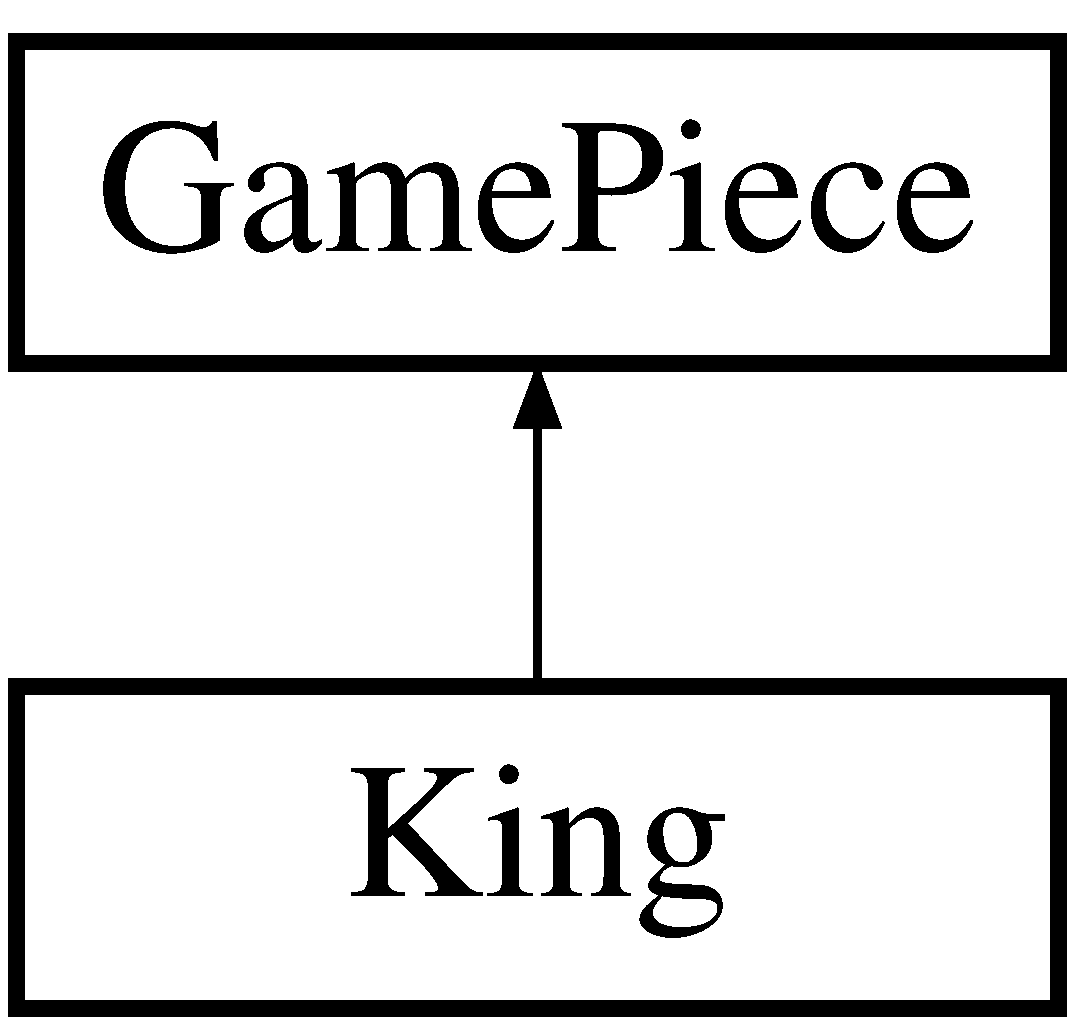
\includegraphics[height=2.000000cm]{class_king}
\end{center}
\end{figure}
\subsection*{Public Member Functions}
\begin{DoxyCompactItemize}
\item 
\hyperlink{class_king_ae132ff90495a95b62097555ed2c069bf}{King} (char)
\item 
virtual char \hyperlink{class_king_a504e6f39d99211c0d69f3dd3a64a8a5e}{get\-Show} ()
\item 
virtual void \hyperlink{class_king_a6d35246db649771c8ef3f5cabd52d239}{val\-Pick} (string, \hyperlink{class_board}{Board} \&, char, char, char \&, int \&)
\item 
virtual bool \hyperlink{class_king_ad20f20db3007c880a5aba1e043968e70}{chk\-Pick} (\hyperlink{class_board}{Board} \&, char, char, char \&, int)
\item 
virtual void \hyperlink{class_king_ac75abcc454291598f9804d3e68817633}{val\-Move} (string, \hyperlink{class_board}{Board} \&, char, char, char, char, int \&, int)
\item 
virtual bool \hyperlink{class_king_ac18d0b1d7f928e0243041999f5a1fb81}{chk\-Move} (\hyperlink{class_board}{Board} \&, char, char, char, int, int)
\end{DoxyCompactItemize}
\subsection*{Additional Inherited Members}


\subsection{Detailed Description}
The \hyperlink{class_king}{King} class represents pieces of the checkerboard which have been 'kinged' Player one (White) has kings that appear as the character 'M' and player two (Black) has kings that appear as the character 'W'. Kings can move backwards and forward on the board, therefore the pointer arithmetic is the same for both the white and black kings. The \hyperlink{class_king}{King} class has its own function for validating it's move, but shares the val\-Pick move with whatever regular checker class is calling it. Aside from that one function, the \hyperlink{class_king}{King} class contains all of the functions responsible for moving the king around the board. 

\subsection{Constructor \& Destructor Documentation}
\hypertarget{class_king_ae132ff90495a95b62097555ed2c069bf}{\index{King@{King}!King@{King}}
\index{King@{King}!King@{King}}
\subsubsection[{King}]{\setlength{\rightskip}{0pt plus 5cm}King\-::\-King (
\begin{DoxyParamCaption}
\item[{char}]{a}
\end{DoxyParamCaption}
)}}\label{class_king_ae132ff90495a95b62097555ed2c069bf}
This function is the constructor for the \hyperlink{class_king}{King} class. The constructor is used to create a king checker. This class inherits from the abstract base class \hyperlink{class_game_piece}{Game\-Piece} whose constructor is called.

\subsection{Member Function Documentation}
\hypertarget{class_king_ac18d0b1d7f928e0243041999f5a1fb81}{\index{King@{King}!chk\-Move@{chk\-Move}}
\index{chk\-Move@{chk\-Move}!King@{King}}
\subsubsection[{chk\-Move}]{\setlength{\rightskip}{0pt plus 5cm}bool King\-::chk\-Move (
\begin{DoxyParamCaption}
\item[{{\bf Board} \&}]{game\-Board, }
\item[{char}]{b\-Piece, }
\item[{char}]{g\-Piece\-O, }
\item[{char}]{k\-Piece\-O, }
\item[{int}]{coord\-S, }
\item[{int}]{coord\-M}
\end{DoxyParamCaption}
)\hspace{0.3cm}{\ttfamily [virtual]}}}\label{class_king_ac18d0b1d7f928e0243041999f5a1fb81}
This function checks to see if the empty game square player two has chosen to move a selected piece to is a valid move. If no piece is being captured the move square must be +7 or +9 squares away from. If a piece is being captured, then the same rules apply in terms of sign but with the numbers +14 and +18. Also the square between the selection and the move needs to contain the opponents game piece in it for it to be valid

Implements \hyperlink{class_game_piece}{Game\-Piece}.

\hypertarget{class_king_ad20f20db3007c880a5aba1e043968e70}{\index{King@{King}!chk\-Pick@{chk\-Pick}}
\index{chk\-Pick@{chk\-Pick}!King@{King}}
\subsubsection[{chk\-Pick}]{\setlength{\rightskip}{0pt plus 5cm}bool King\-::chk\-Pick (
\begin{DoxyParamCaption}
\item[{{\bf Board} \&}]{, }
\item[{char}]{, }
\item[{char}]{, }
\item[{char \&}]{, }
\item[{int}]{}
\end{DoxyParamCaption}
)\hspace{0.3cm}{\ttfamily [virtual]}}}\label{class_king_ad20f20db3007c880a5aba1e043968e70}


Implements \hyperlink{class_game_piece}{Game\-Piece}.

\hypertarget{class_king_a504e6f39d99211c0d69f3dd3a64a8a5e}{\index{King@{King}!get\-Show@{get\-Show}}
\index{get\-Show@{get\-Show}!King@{King}}
\subsubsection[{get\-Show}]{\setlength{\rightskip}{0pt plus 5cm}char King\-::get\-Show (
\begin{DoxyParamCaption}
{}
\end{DoxyParamCaption}
)\hspace{0.3cm}{\ttfamily [virtual]}}}\label{class_king_a504e6f39d99211c0d69f3dd3a64a8a5e}


Implements \hyperlink{class_game_piece}{Game\-Piece}.

\hypertarget{class_king_ac75abcc454291598f9804d3e68817633}{\index{King@{King}!val\-Move@{val\-Move}}
\index{val\-Move@{val\-Move}!King@{King}}
\subsubsection[{val\-Move}]{\setlength{\rightskip}{0pt plus 5cm}void King\-::val\-Move (
\begin{DoxyParamCaption}
\item[{string}]{choice, }
\item[{{\bf Board} \&}]{game\-Board, }
\item[{char}]{g\-Piece, }
\item[{char}]{g\-Piece\-O, }
\item[{char}]{k\-Piece\-O, }
\item[{char}]{b\-Piece, }
\item[{int \&}]{coord\-M, }
\item[{int}]{coord\-S}
\end{DoxyParamCaption}
)\hspace{0.3cm}{\ttfamily [virtual]}}}\label{class_king_ac75abcc454291598f9804d3e68817633}
This function determines which players turn it is and keeps prompting for a coordinate choice until a valid move is made. The valid move is stored in the coord\-M reference variable. In order for a move to be valid the move must be in a forward and diagonal motion of one space if not jumping, and two if a capture is made.

Implements \hyperlink{class_game_piece}{Game\-Piece}.

\hypertarget{class_king_a6d35246db649771c8ef3f5cabd52d239}{\index{King@{King}!val\-Pick@{val\-Pick}}
\index{val\-Pick@{val\-Pick}!King@{King}}
\subsubsection[{val\-Pick}]{\setlength{\rightskip}{0pt plus 5cm}void King\-::val\-Pick (
\begin{DoxyParamCaption}
\item[{string}]{, }
\item[{{\bf Board} \&}]{, }
\item[{char}]{, }
\item[{char}]{, }
\item[{char \&}]{, }
\item[{int \&}]{}
\end{DoxyParamCaption}
)\hspace{0.3cm}{\ttfamily [virtual]}}}\label{class_king_a6d35246db649771c8ef3f5cabd52d239}


Implements \hyperlink{class_game_piece}{Game\-Piece}.



The documentation for this class was generated from the following files\-:\begin{DoxyCompactItemize}
\item 
C\-:/\-Users/\-Alec/\-Desktop/\-Project\-\_\-2/\-Checkers/King.\-h\item 
C\-:/\-Users/\-Alec/\-Desktop/\-Project\-\_\-2/\-Checkers/King.\-cpp\end{DoxyCompactItemize}

\hypertarget{class_queue}{\section{Queue$<$ T $>$ Class Template Reference}
\label{class_queue}\index{Queue$<$ T $>$@{Queue$<$ T $>$}}
}


{\ttfamily \#include \char`\"{}Queue.\-h\char`\"{}}

\subsection*{Public Member Functions}
\begin{DoxyCompactItemize}
\item 
\hyperlink{class_queue_af73bb29c868f7b37f369c668f114bd9f}{Queue} ()
\item 
\hyperlink{class_queue_aa7eef1b427e24555780505de20e9acbc}{$\sim$\-Queue} ()
\item 
\hypertarget{class_queue_aefc2563a28b93c8216ced448158ffebf}{int {\bfseries get\-Size} ()}\label{class_queue_aefc2563a28b93c8216ced448158ffebf}

\item 
void \hyperlink{class_queue_acb12e3d108397a77e412d43cdd0b2836}{clear} ()
\item 
bool \hyperlink{class_queue_a515bd72c9d7d2bc12add78c0d2e79762}{is\-Empty} ()
\item 
void \hyperlink{class_queue_a011d990957da9f9ab6de8956f7d839ea}{enqueue} (T)
\item 
void \hyperlink{class_queue_adb9c19e6c3cec9a761413bf0f8697d7f}{dequeue} (T \&)
\end{DoxyCompactItemize}


\subsection{Detailed Description}
\subsubsection*{template$<$class T$>$class Queue$<$ T $>$}

The \hyperlink{class_queue}{Queue} class is an implementation of a queue data structure. A queue stores and retrieves its elements in a first in first out manner (F\-I\-F\-O). This implementation is dynamic, so the size of the data structure may fluctuate during the program if necessary. 

\subsection{Constructor \& Destructor Documentation}
\hypertarget{class_queue_af73bb29c868f7b37f369c668f114bd9f}{\index{Queue@{Queue}!Queue@{Queue}}
\index{Queue@{Queue}!Queue@{Queue}}
\subsubsection[{Queue}]{\setlength{\rightskip}{0pt plus 5cm}template$<$class T $>$ {\bf Queue}$<$ T $>$\-::{\bf Queue} (
\begin{DoxyParamCaption}
{}
\end{DoxyParamCaption}
)}}\label{class_queue_af73bb29c868f7b37f369c668f114bd9f}
This function is the constructor for the \hyperlink{class_queue}{Queue} class. The function automatically sets the front and rear pointers to null, then sets the size data member to zero.\hypertarget{class_queue_aa7eef1b427e24555780505de20e9acbc}{\index{Queue@{Queue}!$\sim$\-Queue@{$\sim$\-Queue}}
\index{$\sim$\-Queue@{$\sim$\-Queue}!Queue@{Queue}}
\subsubsection[{$\sim$\-Queue}]{\setlength{\rightskip}{0pt plus 5cm}template$<$class T $>$ {\bf Queue}$<$ T $>$\-::$\sim${\bf Queue} (
\begin{DoxyParamCaption}
{}
\end{DoxyParamCaption}
)}}\label{class_queue_aa7eef1b427e24555780505de20e9acbc}
This function is the destructor for the \hyperlink{class_queue}{Queue} class. The function calls the clear function which will delete the contents of the container by popping out all of the elements into a dummy variable

\subsection{Member Function Documentation}
\hypertarget{class_queue_acb12e3d108397a77e412d43cdd0b2836}{\index{Queue@{Queue}!clear@{clear}}
\index{clear@{clear}!Queue@{Queue}}
\subsubsection[{clear}]{\setlength{\rightskip}{0pt plus 5cm}template$<$class T $>$ void {\bf Queue}$<$ T $>$\-::clear (
\begin{DoxyParamCaption}
{}
\end{DoxyParamCaption}
)}}\label{class_queue_acb12e3d108397a77e412d43cdd0b2836}
This function is used in a call from the destructor of this class in order to clear the contents of a queue. A dummy variable is declared to be used as a parameter for the dequeue function which will pop each element out one at a time until the container is empty\hypertarget{class_queue_adb9c19e6c3cec9a761413bf0f8697d7f}{\index{Queue@{Queue}!dequeue@{dequeue}}
\index{dequeue@{dequeue}!Queue@{Queue}}
\subsubsection[{dequeue}]{\setlength{\rightskip}{0pt plus 5cm}template$<$class T$>$ void {\bf Queue}$<$ T $>$\-::dequeue (
\begin{DoxyParamCaption}
\item[{T \&}]{val}
\end{DoxyParamCaption}
)}}\label{class_queue_adb9c19e6c3cec9a761413bf0f8697d7f}
This function is used to dequeue the elements stored inside a queue container If the container is not empty, then the value of the front node is removed from the container and is assigned to the reference variable passed into the function. Finally the size variable is decremented to reflect the changes in the number of elements in the container.\hypertarget{class_queue_a011d990957da9f9ab6de8956f7d839ea}{\index{Queue@{Queue}!enqueue@{enqueue}}
\index{enqueue@{enqueue}!Queue@{Queue}}
\subsubsection[{enqueue}]{\setlength{\rightskip}{0pt plus 5cm}template$<$class T$>$ void {\bf Queue}$<$ T $>$\-::enqueue (
\begin{DoxyParamCaption}
\item[{T}]{val}
\end{DoxyParamCaption}
)}}\label{class_queue_a011d990957da9f9ab6de8956f7d839ea}
This function is used to add elements into the queue. A new node is declared and the value passed into the function is set as the node's value attribute. If the queue is empty then the current node becomes the front and rear. Otherwise the node is added to the rear of the queue container. Finally the size is incremented to keep track of the number of elements.\hypertarget{class_queue_a515bd72c9d7d2bc12add78c0d2e79762}{\index{Queue@{Queue}!is\-Empty@{is\-Empty}}
\index{is\-Empty@{is\-Empty}!Queue@{Queue}}
\subsubsection[{is\-Empty}]{\setlength{\rightskip}{0pt plus 5cm}template$<$class T $>$ bool {\bf Queue}$<$ T $>$\-::is\-Empty (
\begin{DoxyParamCaption}
{}
\end{DoxyParamCaption}
)}}\label{class_queue_a515bd72c9d7d2bc12add78c0d2e79762}
This function is used to determine whether or not a queue is empty. This function is mainly used in the clear function but as well for error checking in the pop function.

The documentation for this class was generated from the following file\-:\begin{DoxyCompactItemize}
\item 
C\-:/\-Users/\-Alec/\-Desktop/\-Project\-\_\-2/\-Checkers/Queue.\-h\end{DoxyCompactItemize}

\hypertarget{class_reg_black}{\section{Reg\-Black Class Reference}
\label{class_reg_black}\index{Reg\-Black@{Reg\-Black}}
}


{\ttfamily \#include \char`\"{}Reg\-Black.\-h\char`\"{}}

Inheritance diagram for Reg\-Black\-:\begin{figure}[H]
\begin{center}
\leavevmode
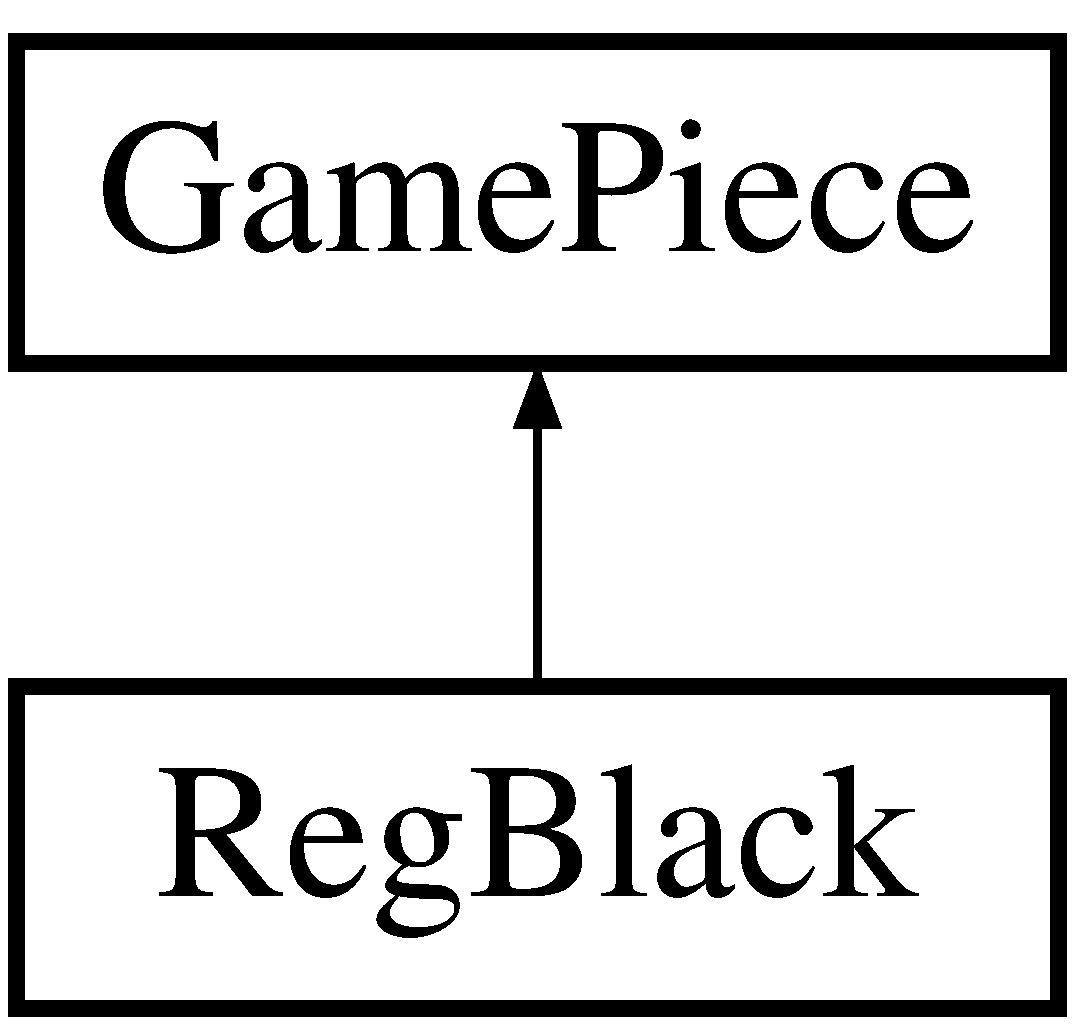
\includegraphics[height=2.000000cm]{class_reg_black}
\end{center}
\end{figure}
\subsection*{Public Member Functions}
\begin{DoxyCompactItemize}
\item 
\hyperlink{class_reg_black_a1c4f49c27b3ecb11b7be7542f1839e92}{Reg\-Black} (char a)
\item 
virtual char \hyperlink{class_reg_black_a443809b57474b3ccb28ad54f8c5a277c}{get\-Show} ()
\item 
virtual void \hyperlink{class_reg_black_abfcac7c66da4b4220899f2af9703a16a}{val\-Pick} (string, \hyperlink{class_board}{Board} \&, char, char, char \&, int \&)
\item 
virtual bool \hyperlink{class_reg_black_a43474ac9c3b2f0c6f016be88ff037c8f}{chk\-Pick} (\hyperlink{class_board}{Board} \&, char, char, char \&, int)
\item 
virtual void \hyperlink{class_reg_black_a5f2764564af69c686e434310e89255d6}{val\-Move} (string, \hyperlink{class_board}{Board} \&, char, char, char, char, int \&, int)
\item 
virtual bool \hyperlink{class_reg_black_a23733f51cc005f551d077857fd9a5bf1}{chk\-Move} (\hyperlink{class_board}{Board} \&, char, char, char, int, int)
\item 
\hypertarget{class_reg_black_a3fff072004c2858dba01d8bbdd9afd1c}{void {\bfseries ai\-Move} (\hyperlink{class_board}{Board} \&, string, string, int \&, int \&)}\label{class_reg_black_a3fff072004c2858dba01d8bbdd9afd1c}

\item 
void \hyperlink{class_reg_black_a54d15e5fa95efc365752e4a1a352e7b9}{chk\-King} (\hyperlink{class_board}{Board} \&, char, char, char, int, int)
\end{DoxyCompactItemize}
\subsection*{Additional Inherited Members}


\subsection{Detailed Description}
The \hyperlink{class_reg_black}{Reg\-Black} class represents the regular black checker which has not been kinged. Since black checkers start at the top of the board where the index values start (element 0 ), regular black checkers can only move in plus + directions. The ascii character 149 which appears as a black bullet is used to represent a black checker piece. The \hyperlink{class_reg_black}{Reg\-Black} class contains all the necessary functions to evaluate moves across the board for black checkers. As with all of the checker piece objects, only one needs to be instantiated for the game, which acts as a key to graining access to the game board. 

\subsection{Constructor \& Destructor Documentation}
\hypertarget{class_reg_black_a1c4f49c27b3ecb11b7be7542f1839e92}{\index{Reg\-Black@{Reg\-Black}!Reg\-Black@{Reg\-Black}}
\index{Reg\-Black@{Reg\-Black}!RegBlack@{Reg\-Black}}
\subsubsection[{Reg\-Black}]{\setlength{\rightskip}{0pt plus 5cm}Reg\-Black\-::\-Reg\-Black (
\begin{DoxyParamCaption}
\item[{char}]{a}
\end{DoxyParamCaption}
)}}\label{class_reg_black_a1c4f49c27b3ecb11b7be7542f1839e92}
This function is the constructor for the \hyperlink{class_reg_black}{Reg\-Black} class. The constructor is used to create a regular black checker. This class inherits from the abstract base class \hyperlink{class_game_piece}{Game\-Piece} whose constructor is called.

\subsection{Member Function Documentation}
\hypertarget{class_reg_black_a54d15e5fa95efc365752e4a1a352e7b9}{\index{Reg\-Black@{Reg\-Black}!chk\-King@{chk\-King}}
\index{chk\-King@{chk\-King}!RegBlack@{Reg\-Black}}
\subsubsection[{chk\-King}]{\setlength{\rightskip}{0pt plus 5cm}void Reg\-Black\-::chk\-King (
\begin{DoxyParamCaption}
\item[{{\bf Board} \&}]{game\-Board, }
\item[{char}]{g\-Piece, }
\item[{char}]{k\-Piece, }
\item[{char}]{g\-Piece\-O, }
\item[{int}]{p1\-Pieces, }
\item[{int}]{p2\-Pieces}
\end{DoxyParamCaption}
)}}\label{class_reg_black_a54d15e5fa95efc365752e4a1a352e7b9}
This function checks to see if player two has made one of their pieces to the opposite side of the board. If so the square of the board is assigned the character 'W' representing a king and the program lets the users know of the change.\hypertarget{class_reg_black_a23733f51cc005f551d077857fd9a5bf1}{\index{Reg\-Black@{Reg\-Black}!chk\-Move@{chk\-Move}}
\index{chk\-Move@{chk\-Move}!RegBlack@{Reg\-Black}}
\subsubsection[{chk\-Move}]{\setlength{\rightskip}{0pt plus 5cm}bool Reg\-Black\-::chk\-Move (
\begin{DoxyParamCaption}
\item[{{\bf Board} \&}]{game\-Board, }
\item[{char}]{b\-Piece, }
\item[{char}]{g\-Piece\-O, }
\item[{char}]{k\-Piece\-O, }
\item[{int}]{coord\-S, }
\item[{int}]{coord\-M}
\end{DoxyParamCaption}
)\hspace{0.3cm}{\ttfamily [virtual]}}}\label{class_reg_black_a23733f51cc005f551d077857fd9a5bf1}
This function checks to see if the empty game square player two has chosen to move a selected piece to is a valid move. If no piece is being captured the move square must be +7 or +9 squares away from. If a piece is being captured, then the same rules apply in terms of sign but with the numbers +14 and +18. Also the square between the selection and the move needs to contain the opponents game piece in it for it to be valid

Implements \hyperlink{class_game_piece}{Game\-Piece}.

\hypertarget{class_reg_black_a43474ac9c3b2f0c6f016be88ff037c8f}{\index{Reg\-Black@{Reg\-Black}!chk\-Pick@{chk\-Pick}}
\index{chk\-Pick@{chk\-Pick}!RegBlack@{Reg\-Black}}
\subsubsection[{chk\-Pick}]{\setlength{\rightskip}{0pt plus 5cm}bool Reg\-Black\-::chk\-Pick (
\begin{DoxyParamCaption}
\item[{{\bf Board} \&}]{game\-Board, }
\item[{char}]{g\-Piece, }
\item[{char}]{k\-Piece, }
\item[{char \&}]{used, }
\item[{int}]{element}
\end{DoxyParamCaption}
)\hspace{0.3cm}{\ttfamily [virtual]}}}\label{class_reg_black_a43474ac9c3b2f0c6f016be88ff037c8f}
This function checks the selection made by a player and determines if it is valid. In order for the selection to be valid the array element of that coordinate must contain that particular player's piece in it.

Implements \hyperlink{class_game_piece}{Game\-Piece}.

\hypertarget{class_reg_black_a443809b57474b3ccb28ad54f8c5a277c}{\index{Reg\-Black@{Reg\-Black}!get\-Show@{get\-Show}}
\index{get\-Show@{get\-Show}!RegBlack@{Reg\-Black}}
\subsubsection[{get\-Show}]{\setlength{\rightskip}{0pt plus 5cm}char Reg\-Black\-::get\-Show (
\begin{DoxyParamCaption}
{}
\end{DoxyParamCaption}
)\hspace{0.3cm}{\ttfamily [virtual]}}}\label{class_reg_black_a443809b57474b3ccb28ad54f8c5a277c}
Accessor function for the regular black checker, returns the char variable named show, value of 149 representing a black bullet like character

Implements \hyperlink{class_game_piece}{Game\-Piece}.

\hypertarget{class_reg_black_a5f2764564af69c686e434310e89255d6}{\index{Reg\-Black@{Reg\-Black}!val\-Move@{val\-Move}}
\index{val\-Move@{val\-Move}!RegBlack@{Reg\-Black}}
\subsubsection[{val\-Move}]{\setlength{\rightskip}{0pt plus 5cm}void Reg\-Black\-::val\-Move (
\begin{DoxyParamCaption}
\item[{string}]{choice, }
\item[{{\bf Board} \&}]{game\-Board, }
\item[{char}]{g\-Piece, }
\item[{char}]{g\-Piece\-O, }
\item[{char}]{k\-Piece\-O, }
\item[{char}]{b\-Piece, }
\item[{int \&}]{coord\-M, }
\item[{int}]{coord\-S}
\end{DoxyParamCaption}
)\hspace{0.3cm}{\ttfamily [virtual]}}}\label{class_reg_black_a5f2764564af69c686e434310e89255d6}
This function determines which players turn it is and keeps prompting for a coordinate choice until a valid move is made. The valid move is stored in the coord\-M reference variable. In order for a move to be valid the move must be in a forward and diagonal motion of one space if not jumping, and two if a capture is made.

Implements \hyperlink{class_game_piece}{Game\-Piece}.

\hypertarget{class_reg_black_abfcac7c66da4b4220899f2af9703a16a}{\index{Reg\-Black@{Reg\-Black}!val\-Pick@{val\-Pick}}
\index{val\-Pick@{val\-Pick}!RegBlack@{Reg\-Black}}
\subsubsection[{val\-Pick}]{\setlength{\rightskip}{0pt plus 5cm}void Reg\-Black\-::val\-Pick (
\begin{DoxyParamCaption}
\item[{string}]{choice, }
\item[{{\bf Board} \&}]{game\-Board, }
\item[{char}]{g\-Piece, }
\item[{char}]{k\-Piece, }
\item[{char \&}]{used, }
\item[{int \&}]{coord\-S}
\end{DoxyParamCaption}
)\hspace{0.3cm}{\ttfamily [virtual]}}}\label{class_reg_black_abfcac7c66da4b4220899f2af9703a16a}
This function determines which players turn it is and keeps prompting for a coordinate choice until a valid pick is made. The valid pick is stored in the coord\-S reference variable. This is one of two functions responsible for validating input in terms of what is legal within the rules of the game, the other is val\-Move

Implements \hyperlink{class_game_piece}{Game\-Piece}.



The documentation for this class was generated from the following files\-:\begin{DoxyCompactItemize}
\item 
C\-:/\-Users/\-Alec/\-Desktop/\-Project\-\_\-2/\-Checkers/Reg\-Black.\-h\item 
C\-:/\-Users/\-Alec/\-Desktop/\-Project\-\_\-2/\-Checkers/Reg\-Black.\-cpp\end{DoxyCompactItemize}

\hypertarget{class_reg_white}{\section{Reg\-White Class Reference}
\label{class_reg_white}\index{Reg\-White@{Reg\-White}}
}


{\ttfamily \#include \char`\"{}Reg\-White.\-h\char`\"{}}

Inheritance diagram for Reg\-White\-:\begin{figure}[H]
\begin{center}
\leavevmode
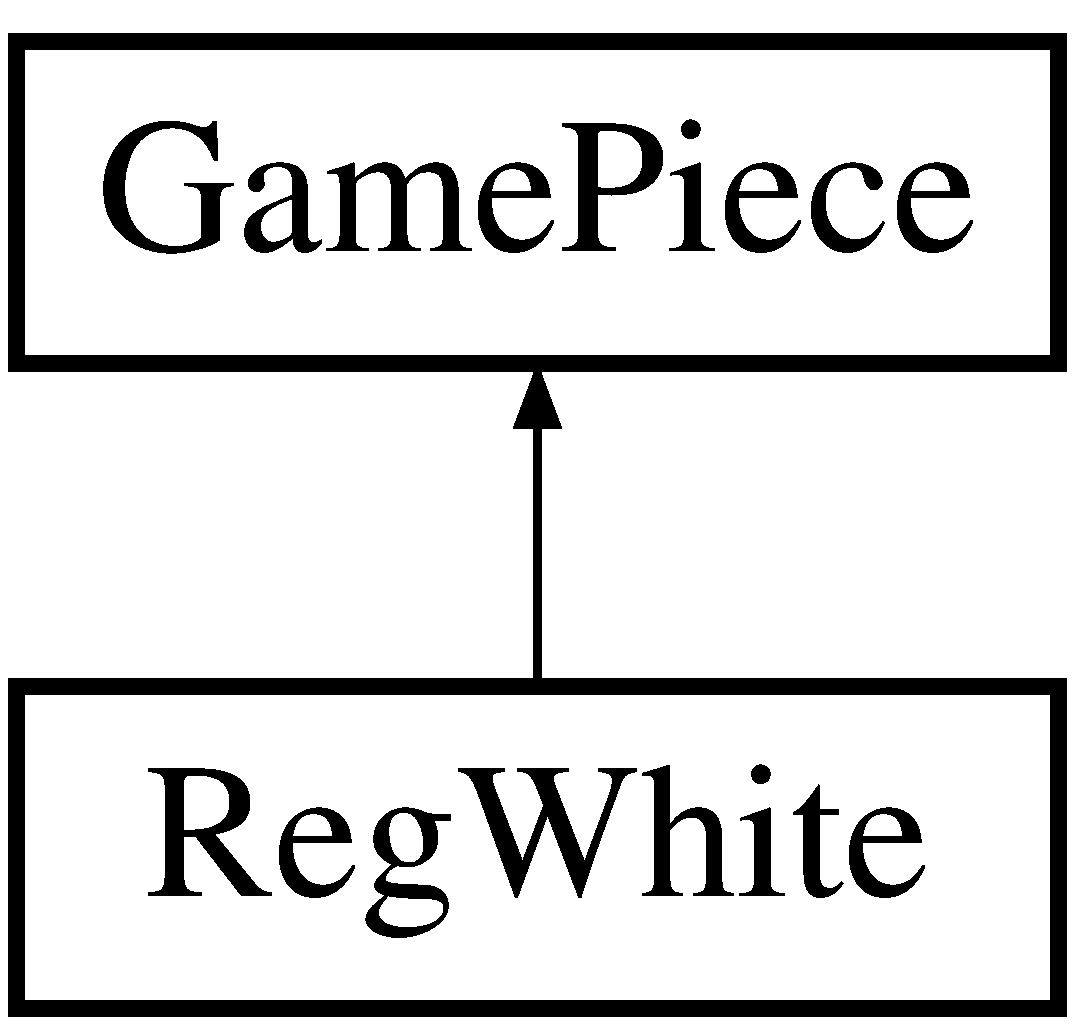
\includegraphics[height=2.000000cm]{class_reg_white}
\end{center}
\end{figure}
\subsection*{Public Member Functions}
\begin{DoxyCompactItemize}
\item 
\hyperlink{class_reg_white_a2a424aed051c97e73ffa03ac7a9b9ec0}{Reg\-White} (char a)
\item 
virtual char \hyperlink{class_reg_white_aa59f0cfb60c36f631004242c33dfcabc}{get\-Show} ()
\item 
virtual void \hyperlink{class_reg_white_a7995b3b0df425a15c9da2bf8be8dca3a}{val\-Pick} (string, \hyperlink{class_board}{Board} \&, char, char, char \&, int \&)
\item 
virtual bool \hyperlink{class_reg_white_a298051d178de6cd50689ad43e8bc9f04}{chk\-Pick} (\hyperlink{class_board}{Board} \&, char, char, char \&, int)
\item 
virtual void \hyperlink{class_reg_white_a9bdb0787be549a35da2afe05950ba2f1}{val\-Move} (string, \hyperlink{class_board}{Board} \&, char, char, char, char, int \&, int)
\item 
virtual bool \hyperlink{class_reg_white_acacc51249fc17deb0e1f50cc9c09d068}{chk\-Move} (\hyperlink{class_board}{Board} \&, char, char, char, int, int)
\item 
void \hyperlink{class_reg_white_a6062b358e5da3b86ccfc3136664daaaf}{chk\-King} (\hyperlink{class_board}{Board} \&, char, char, char, int, int)
\end{DoxyCompactItemize}
\subsection*{Additional Inherited Members}


\subsection{Detailed Description}
The \hyperlink{class_reg_white}{Reg\-White} class represents the regular white checker which has not been kinged. Since white checkers start at the bottom of the board where the index values approach their max regular black checkers can only move in minus -\/ directions. An uppercase 'O' character is used to represent a white checker piece. The \hyperlink{class_reg_white}{Reg\-White} class contains all the necessary functions to evaluate moves across the board for white checkers. As with all of the checker piece objects, only one needs to be instantiated for the game, which acts as a key to gaining access to the game board. 

\subsection{Constructor \& Destructor Documentation}
\hypertarget{class_reg_white_a2a424aed051c97e73ffa03ac7a9b9ec0}{\index{Reg\-White@{Reg\-White}!Reg\-White@{Reg\-White}}
\index{Reg\-White@{Reg\-White}!RegWhite@{Reg\-White}}
\subsubsection[{Reg\-White}]{\setlength{\rightskip}{0pt plus 5cm}Reg\-White\-::\-Reg\-White (
\begin{DoxyParamCaption}
\item[{char}]{a}
\end{DoxyParamCaption}
)}}\label{class_reg_white_a2a424aed051c97e73ffa03ac7a9b9ec0}
This function is the constructor for the \hyperlink{class_reg_white}{Reg\-White} class. The constructor is used to create a regular white checker. This class inherits from the abstract base class \hyperlink{class_game_piece}{Game\-Piece} whose constructor is called.

\subsection{Member Function Documentation}
\hypertarget{class_reg_white_a6062b358e5da3b86ccfc3136664daaaf}{\index{Reg\-White@{Reg\-White}!chk\-King@{chk\-King}}
\index{chk\-King@{chk\-King}!RegWhite@{Reg\-White}}
\subsubsection[{chk\-King}]{\setlength{\rightskip}{0pt plus 5cm}void Reg\-White\-::chk\-King (
\begin{DoxyParamCaption}
\item[{{\bf Board} \&}]{game\-Board, }
\item[{char}]{g\-Piece, }
\item[{char}]{k\-Piece, }
\item[{char}]{g\-Piece\-O, }
\item[{int}]{p1\-Pieces, }
\item[{int}]{p2\-Pieces}
\end{DoxyParamCaption}
)}}\label{class_reg_white_a6062b358e5da3b86ccfc3136664daaaf}
This function checks to see if player one has made one of their pieces to the opposite side of the board. If so the square of the board is assigned the character 'W' representing a king and the program lets the users know of the change.\hypertarget{class_reg_white_acacc51249fc17deb0e1f50cc9c09d068}{\index{Reg\-White@{Reg\-White}!chk\-Move@{chk\-Move}}
\index{chk\-Move@{chk\-Move}!RegWhite@{Reg\-White}}
\subsubsection[{chk\-Move}]{\setlength{\rightskip}{0pt plus 5cm}bool Reg\-White\-::chk\-Move (
\begin{DoxyParamCaption}
\item[{{\bf Board} \&}]{game\-Board, }
\item[{char}]{b\-Piece, }
\item[{char}]{g\-Piece\-O, }
\item[{char}]{k\-Piece\-O, }
\item[{int}]{coord\-S, }
\item[{int}]{coord\-M}
\end{DoxyParamCaption}
)\hspace{0.3cm}{\ttfamily [virtual]}}}\label{class_reg_white_acacc51249fc17deb0e1f50cc9c09d068}
This function checks to see if the empty game square player two has chosen to move a selected piece to is a valid move. If no piece is being captured the move square must be +7 or +9 squares away from. If a piece is being captured, then the same rules apply in terms of sign but with the numbers +14 and +18. Also the square between the selection and the move needs to contain the opponents game piece in it for it to be valid

Implements \hyperlink{class_game_piece}{Game\-Piece}.

\hypertarget{class_reg_white_a298051d178de6cd50689ad43e8bc9f04}{\index{Reg\-White@{Reg\-White}!chk\-Pick@{chk\-Pick}}
\index{chk\-Pick@{chk\-Pick}!RegWhite@{Reg\-White}}
\subsubsection[{chk\-Pick}]{\setlength{\rightskip}{0pt plus 5cm}bool Reg\-White\-::chk\-Pick (
\begin{DoxyParamCaption}
\item[{{\bf Board} \&}]{game\-Board, }
\item[{char}]{g\-Piece, }
\item[{char}]{k\-Piece, }
\item[{char \&}]{used, }
\item[{int}]{element}
\end{DoxyParamCaption}
)\hspace{0.3cm}{\ttfamily [virtual]}}}\label{class_reg_white_a298051d178de6cd50689ad43e8bc9f04}
This function checks the selection made by a player and determines if it is valid. In order for the selection to be valid the array element of that coordinate must contain that particular player's piece in it.

Implements \hyperlink{class_game_piece}{Game\-Piece}.

\hypertarget{class_reg_white_aa59f0cfb60c36f631004242c33dfcabc}{\index{Reg\-White@{Reg\-White}!get\-Show@{get\-Show}}
\index{get\-Show@{get\-Show}!RegWhite@{Reg\-White}}
\subsubsection[{get\-Show}]{\setlength{\rightskip}{0pt plus 5cm}char Reg\-White\-::get\-Show (
\begin{DoxyParamCaption}
{}
\end{DoxyParamCaption}
)\hspace{0.3cm}{\ttfamily [virtual]}}}\label{class_reg_white_aa59f0cfb60c36f631004242c33dfcabc}
Accessor function for the regular black checker, returns the char variable named show, value of 149 representing a black bullet like character

Implements \hyperlink{class_game_piece}{Game\-Piece}.

\hypertarget{class_reg_white_a9bdb0787be549a35da2afe05950ba2f1}{\index{Reg\-White@{Reg\-White}!val\-Move@{val\-Move}}
\index{val\-Move@{val\-Move}!RegWhite@{Reg\-White}}
\subsubsection[{val\-Move}]{\setlength{\rightskip}{0pt plus 5cm}void Reg\-White\-::val\-Move (
\begin{DoxyParamCaption}
\item[{string}]{choice, }
\item[{{\bf Board} \&}]{game\-Board, }
\item[{char}]{g\-Piece, }
\item[{char}]{g\-Piece\-O, }
\item[{char}]{k\-Piece\-O, }
\item[{char}]{b\-Piece, }
\item[{int \&}]{coord\-M, }
\item[{int}]{coord\-S}
\end{DoxyParamCaption}
)\hspace{0.3cm}{\ttfamily [virtual]}}}\label{class_reg_white_a9bdb0787be549a35da2afe05950ba2f1}
This function determines which players turn it is and keeps prompting for a coordinate choice until a valid move is made. The valid move is stored in the coord\-M reference variable. In order for a move to be valid the move must be in a forward and diagonal motion of one space if not jumping, and two if a capture is made.

Implements \hyperlink{class_game_piece}{Game\-Piece}.

\hypertarget{class_reg_white_a7995b3b0df425a15c9da2bf8be8dca3a}{\index{Reg\-White@{Reg\-White}!val\-Pick@{val\-Pick}}
\index{val\-Pick@{val\-Pick}!RegWhite@{Reg\-White}}
\subsubsection[{val\-Pick}]{\setlength{\rightskip}{0pt plus 5cm}void Reg\-White\-::val\-Pick (
\begin{DoxyParamCaption}
\item[{string}]{choice, }
\item[{{\bf Board} \&}]{game\-Board, }
\item[{char}]{g\-Piece, }
\item[{char}]{k\-Piece, }
\item[{char \&}]{used, }
\item[{int \&}]{coord\-S}
\end{DoxyParamCaption}
)\hspace{0.3cm}{\ttfamily [virtual]}}}\label{class_reg_white_a7995b3b0df425a15c9da2bf8be8dca3a}
This function determines which players turn it is and keeps prompting for a coordinate choice until a valid pick is made. The valid pick is stored in the coord\-S reference variable. This is one of two functions responsible for validating input in terms of what is legal within the rules of the game, the other is val\-Move

Implements \hyperlink{class_game_piece}{Game\-Piece}.



The documentation for this class was generated from the following files\-:\begin{DoxyCompactItemize}
\item 
C\-:/\-Users/\-Alec/\-Desktop/\-Project\-\_\-2/\-Checkers/Reg\-White.\-h\item 
C\-:/\-Users/\-Alec/\-Desktop/\-Project\-\_\-2/\-Checkers/Reg\-White.\-cpp\end{DoxyCompactItemize}

\hypertarget{class_stack}{\section{Stack$<$ T $>$ Class Template Reference}
\label{class_stack}\index{Stack$<$ T $>$@{Stack$<$ T $>$}}
}
\subsection*{Public Member Functions}
\begin{DoxyCompactItemize}
\item 
\hypertarget{class_stack_ad0db0d9b249e871bb7504ed89a99d3a7}{bool {\bfseries is\-Empty} ()}\label{class_stack_ad0db0d9b249e871bb7504ed89a99d3a7}

\item 
\hypertarget{class_stack_a23b04908bc297e161d12aa75f5382bfd}{void {\bfseries push} (T)}\label{class_stack_a23b04908bc297e161d12aa75f5382bfd}

\item 
\hypertarget{class_stack_aed15c5e2145d9a9f8d5eddbed8b24b86}{void {\bfseries pop} (T \&)}\label{class_stack_aed15c5e2145d9a9f8d5eddbed8b24b86}

\end{DoxyCompactItemize}


The documentation for this class was generated from the following file\-:\begin{DoxyCompactItemize}
\item 
C\-:/\-Users/\-Alec/\-Desktop/\-Project\-\_\-2/\-Checkers/Stack.\-h\end{DoxyCompactItemize}

\hypertarget{class_state}{\section{State Class Reference}
\label{class_state}\index{State@{State}}
}


{\ttfamily \#include \char`\"{}State.\-h\char`\"{}}

Inheritance diagram for State\-:\begin{figure}[H]
\begin{center}
\leavevmode
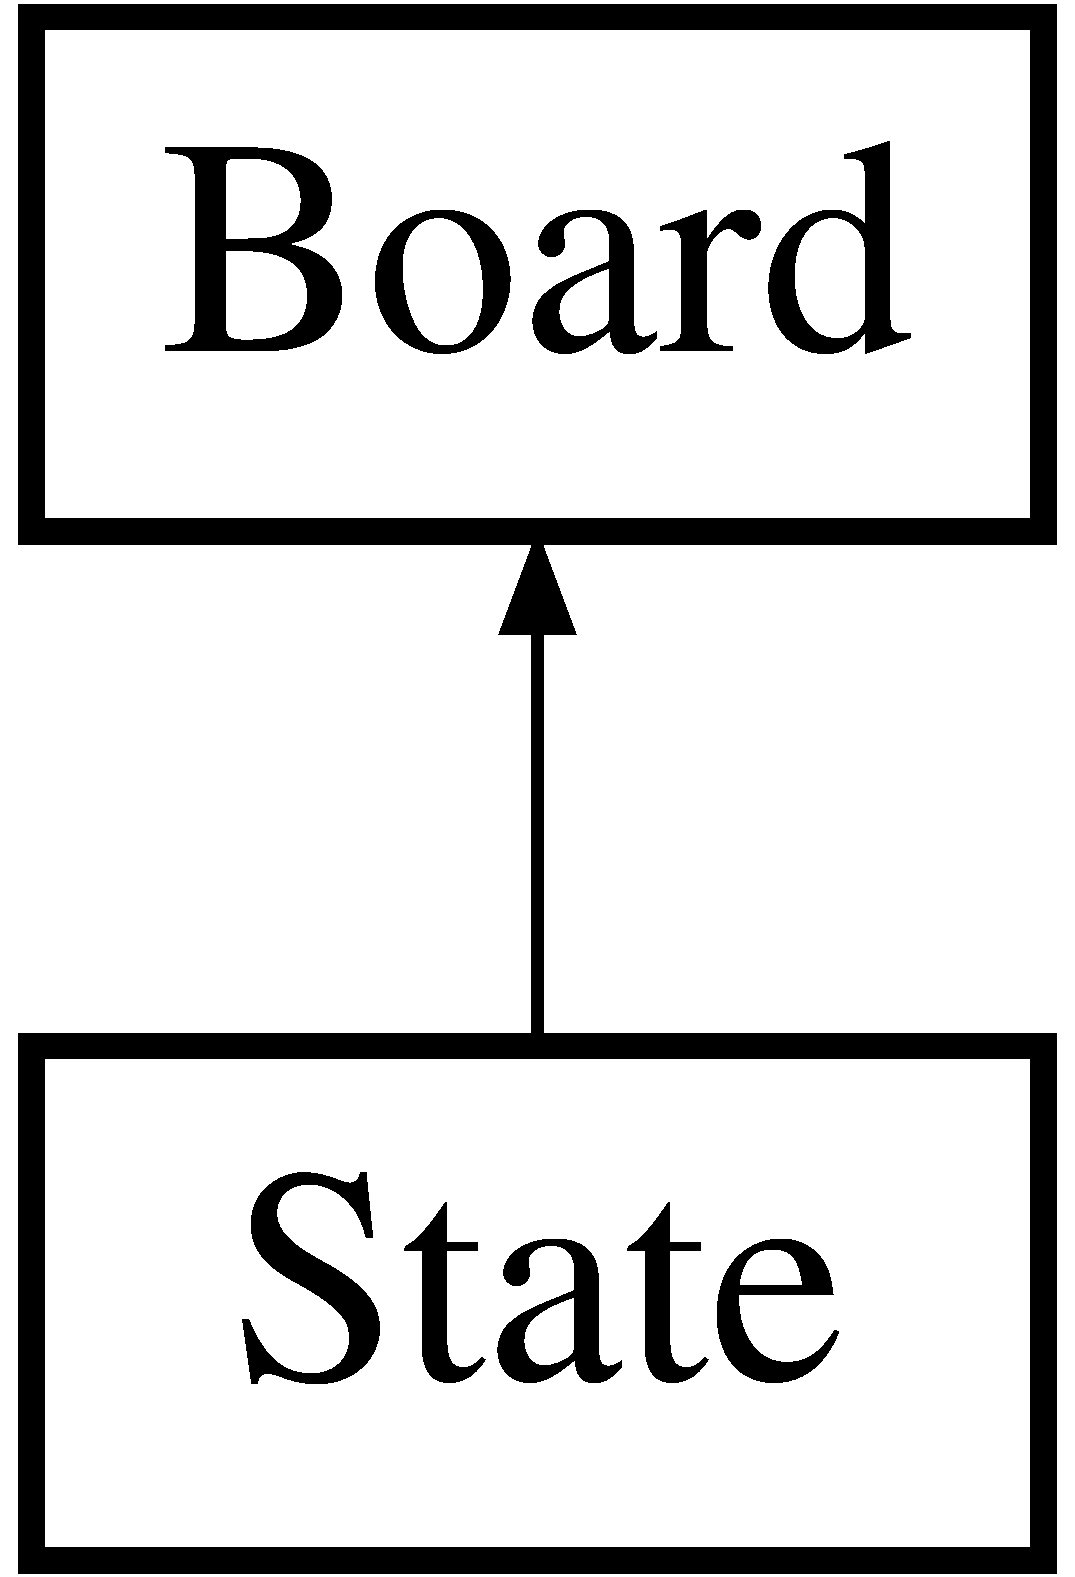
\includegraphics[height=2.000000cm]{class_state}
\end{center}
\end{figure}
\subsection*{Public Member Functions}
\begin{DoxyCompactItemize}
\item 
\hyperlink{class_state_aebfd8b6e0c1c801bcef2160ce1a4aa7f}{State} (\hyperlink{class_board}{Board} \&)
\item 
\hyperlink{class_state_a5648beca719c17700abdf3d7e09298a1}{State} (\hyperlink{class_board}{Board} \&, std\-::string, std\-::string, int)
\item 
int \hyperlink{class_state_a12df9c21402d4f595904c91d2753e17a}{get\-Choice} (\hyperlink{class_state}{State} $\ast$, std\-::string, int)
\item 
void \hyperlink{class_state_a2cd79fa626e83ed7b9aee2cb1f111f99}{remove} (\hyperlink{class_state}{State} \&, int, int)
\item 
void \hyperlink{class_state_a70f163051bd4e35f510b232a1dbd4d16}{print} ()
\item 
float \hyperlink{class_state_a399000f09fffa8b80e3c6145bfb15c14}{utility} ()
\item 
\hyperlink{class_state}{State} \hyperlink{class_state_a25e7e4763a808d30065fc81c933e5518}{operator=} (\hyperlink{class_state}{State} \&)
\end{DoxyCompactItemize}
\subsection*{Friends}
\begin{DoxyCompactItemize}
\item 
\hypertarget{class_state_ab195efc2372da59d716bafc1ce54f7ed}{class {\bfseries Game\-Tree}}\label{class_state_ab195efc2372da59d716bafc1ce54f7ed}

\end{DoxyCompactItemize}
\subsection*{Additional Inherited Members}


\subsection{Detailed Description}
The \hyperlink{class_state}{State} class represents the state of the game at a given position. This classes primary purpose is for use in the A\-I's decision. The \hyperlink{class_game_tree}{Game\-Tree} class creates a tree by filling it up with \hyperlink{class_state}{State} objects representing all the possible legal moves for each player starting from a given position, up to a certain depth limit. The state class inherits from the \hyperlink{class_board}{Board} class and uses its copy constructor in the derived constructor call and then makes the appropriate changes for each legal move. Then the utility function is applied to give the instance being declared a numeric score to be used in the minimax decision. 

\subsection{Constructor \& Destructor Documentation}
\hypertarget{class_state_aebfd8b6e0c1c801bcef2160ce1a4aa7f}{\index{State@{State}!State@{State}}
\index{State@{State}!State@{State}}
\subsubsection[{State}]{\setlength{\rightskip}{0pt plus 5cm}State\-::\-State (
\begin{DoxyParamCaption}
\item[{{\bf Board} \&}]{a}
\end{DoxyParamCaption}
)}}\label{class_state_aebfd8b6e0c1c801bcef2160ce1a4aa7f}
Name\-: Alec Farfan Date\-: 06/03/14 Purpose\-: Functions of the \hyperlink{class_state}{State} class This function is the default constructor for the \hyperlink{class_state}{State} class. A \hyperlink{class_board}{Board} object is passed into the function and then is passed to the copy constructor of the base class.\hypertarget{class_state_a5648beca719c17700abdf3d7e09298a1}{\index{State@{State}!State@{State}}
\index{State@{State}!State@{State}}
\subsubsection[{State}]{\setlength{\rightskip}{0pt plus 5cm}State\-::\-State (
\begin{DoxyParamCaption}
\item[{{\bf Board} \&}]{game\-Board, }
\item[{std\-::string}]{coord\-S, }
\item[{std\-::string}]{coord\-M, }
\item[{int}]{depth}
\end{DoxyParamCaption}
)}}\label{class_state_a5648beca719c17700abdf3d7e09298a1}
This function is the constructor of the \hyperlink{class_state}{State} class used in the generation of the game tree. The \hyperlink{class_board}{Board} object passed into the parameters is then passed to the copy constructor of the base class. The appropriate changes in the board are immediately applied to the new \hyperlink{class_state}{State} object's game board. Finally the utility function is applied giving the game state a numeric score.

\subsection{Member Function Documentation}
\hypertarget{class_state_a12df9c21402d4f595904c91d2753e17a}{\index{State@{State}!get\-Choice@{get\-Choice}}
\index{get\-Choice@{get\-Choice}!State@{State}}
\subsubsection[{get\-Choice}]{\setlength{\rightskip}{0pt plus 5cm}int State\-::get\-Choice (
\begin{DoxyParamCaption}
\item[{{\bf State} $\ast$}]{obj, }
\item[{std\-::string}]{coord, }
\item[{int}]{index}
\end{DoxyParamCaption}
)}}\label{class_state_a12df9c21402d4f595904c91d2753e17a}
This function reads in a letter/number coordinate choice from the user which is then copied into a character array to be manipulated and tested for validity. The type of validity this function is responsible for checking is in terms of data format ie. proper size, proper letter/number entry, ect. The val\-Choice and val\-Move functions are responsible for testing validity in terms of what is legal in the game of checkers.\hypertarget{class_state_a25e7e4763a808d30065fc81c933e5518}{\index{State@{State}!operator=@{operator=}}
\index{operator=@{operator=}!State@{State}}
\subsubsection[{operator=}]{\setlength{\rightskip}{0pt plus 5cm}{\bf State} State\-::operator= (
\begin{DoxyParamCaption}
\item[{{\bf State} \&}]{right}
\end{DoxyParamCaption}
)}}\label{class_state_a25e7e4763a808d30065fc81c933e5518}
This function overloads the assignment operator '=' for the \hyperlink{class_state}{State} class. When an assignment is made from one \hyperlink{class_state}{State} object to another only the character array representing the game board is copied over.\hypertarget{class_state_a70f163051bd4e35f510b232a1dbd4d16}{\index{State@{State}!print@{print}}
\index{print@{print}!State@{State}}
\subsubsection[{print}]{\setlength{\rightskip}{0pt plus 5cm}void State\-::print (
\begin{DoxyParamCaption}
{}
\end{DoxyParamCaption}
)}}\label{class_state_a70f163051bd4e35f510b232a1dbd4d16}
This function is not used in the game of checkers, it is primarily for testing purposes. The function prints the array representing the game board of the \hyperlink{class_state}{State} object calling it. Calling this function while the tree is generating at a certain depth gives a good view of what moves are available\hypertarget{class_state_a2cd79fa626e83ed7b9aee2cb1f111f99}{\index{State@{State}!remove@{remove}}
\index{remove@{remove}!State@{State}}
\subsubsection[{remove}]{\setlength{\rightskip}{0pt plus 5cm}void State\-::remove (
\begin{DoxyParamCaption}
\item[{{\bf State} \&}]{game\-Board, }
\item[{int}]{coord\-S, }
\item[{int}]{coord\-M}
\end{DoxyParamCaption}
)}}\label{class_state_a2cd79fa626e83ed7b9aee2cb1f111f99}
This function is used to remove game pieces that have been hopped over in the generation of a game state. This function overrides the remove function from the base class hence the \hyperlink{class_state}{State} object passed in as the first parameter\hypertarget{class_state_a399000f09fffa8b80e3c6145bfb15c14}{\index{State@{State}!utility@{utility}}
\index{utility@{utility}!State@{State}}
\subsubsection[{utility}]{\setlength{\rightskip}{0pt plus 5cm}float State\-::utility (
\begin{DoxyParamCaption}
{}
\end{DoxyParamCaption}
)}}\label{class_state_a399000f09fffa8b80e3c6145bfb15c14}
This function calculates and assigns a numeric score for each game state that is generated. All the functions used to improve heuristics are called from this function, contributing to the final score of the game state. After the total is calculated the score is stored in the \hyperlink{class_state}{State} object.

The documentation for this class was generated from the following files\-:\begin{DoxyCompactItemize}
\item 
C\-:/\-Users/\-Alec/\-Desktop/\-Project\-\_\-2/\-Checkers/State.\-h\item 
C\-:/\-Users/\-Alec/\-Desktop/\-Project\-\_\-2/\-Checkers/State.\-cpp\end{DoxyCompactItemize}

%--- End generated contents ---

% Index
\newpage
\phantomsection
\addcontentsline{toc}{chapter}{Index}
\printindex

\end{document}
